% This LaTeX was auto-generated from MATLAB code.
% To make changes, update the MATLAB code and export to LaTeX again.

\documentclass{article}

\usepackage[utf8]{inputenc}
\usepackage[T1]{fontenc}
\usepackage{lmodern}
\usepackage{graphicx}
\usepackage{color}
\usepackage{hyperref}
\usepackage{amsmath}
\usepackage{amsfonts}
\usepackage{epstopdf}
\usepackage[table]{xcolor}
\usepackage{matlab}

\sloppy
\epstopdfsetup{outdir=./}
\graphicspath{ {./Week1_Assignment_images/} }

\begin{document}

\begin{par}
\begin{flushleft}
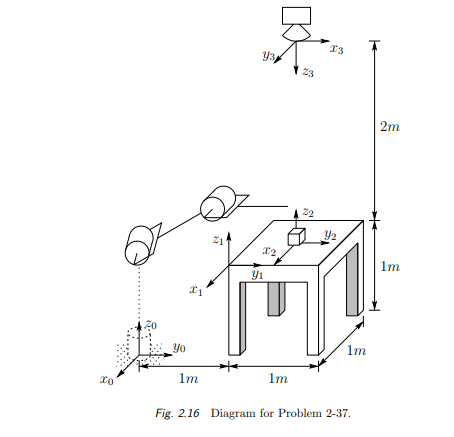
\includegraphics[width=\maxwidth{45.55945810336177em}]{image_0}
\end{flushleft}
\end{par}

\begin{par}
\begin{flushleft}
Consider the diagram of Figure 2.16. A robot is set up 1 meter from a table. The table top is 1 meter high and 1 meter square. A frame o1x1y1z1 is fixed to the edge of the table as shown. A cube measuring 20 cm on a side is placed in the center of the table with frame o2x2y2z2 established at the center of the cube as shown. A camera is situated directly above the center of the block 2m above the table top with frame o3x3y3z3 attached as shown. Find the homogeneous transformations relating each of these frames to the base frame o0x0y0z0. Find the homogeneous transformation relating the frame o2x2y2z2 to the camera frame o3x3y3z3. 
\end{flushleft}
\end{par}

\begin{par}
\begin{flushleft}
The transformations between frames 0 and 1, and 1 and 2 are easily shown through translations only. However the transformations between 2 and 3 requires rotations. 
\end{flushleft}
\end{par}

\begin{matlabcode}
syms theta

H_0_1 = [1 0 0 0; 0 1 0 1; 0 0 1 1; 0 0 0 1]
\end{matlabcode}
\begin{matlaboutput}
H_0_1 = 4x4    
     1     0     0     0
     0     1     0     1
     0     0     1     1
     0     0     0     1

\end{matlaboutput}
\begin{matlabcode}
H_1_2 = [1 0 0 -0.5; 0 1 0 0.5; 0 0 1 0; 0 0 0 1]
\end{matlabcode}
\begin{matlaboutput}
H_1_2 = 4x4    
    1.0000         0         0   -0.5000
         0    1.0000         0    0.5000
         0         0    1.0000         0
         0         0         0    1.0000

\end{matlaboutput}
\begin{matlabcode}

\end{matlabcode}

\begin{par}
\begin{flushleft}
 We can match the rotation between frames 2 and 3 with a 180 degree rotation in y followed by a 90 degree rotation in z.
\end{flushleft}
\end{par}

\begin{matlabcode}
H_2_3_Translation = [1 0 0 0; 0 1 0 0; 0 0 1 2; 0 0 0 1]
\end{matlabcode}
\begin{matlaboutput}
H_2_3_Translation = 4x4    
     1     0     0     0
     0     1     0     0
     0     0     1     2
     0     0     0     1

\end{matlaboutput}
\begin{matlabcode}

H_y_rot = [cosd(theta) 0 sind(theta) 0; 0 1 0 0; -sind(theta) 0 cosd(theta) 0; 0 0 0 1]
\end{matlabcode}
\begin{matlabsymbolicoutput}
H\_y\_rot = 

\hskip1em $\displaystyle \left(\begin{array}{cccc}
\cos \left(\frac{\pi \,\theta }{180}\right) & 0 & \sin \left(\frac{\pi \,\theta }{180}\right) & 0\\
0 & 1 & 0 & 0\\
-\sin \left(\frac{\pi \,\theta }{180}\right) & 0 & \cos \left(\frac{\pi \,\theta }{180}\right) & 0\\
0 & 0 & 0 & 1
\end{array}\right)$
\end{matlabsymbolicoutput}
\begin{matlabcode}
H_z_rot = [cosd(theta) -sind(theta) 0 0; sind(theta) cosd(theta) 0 0; 0 0 1 0; 0 0 0 1]
\end{matlabcode}
\begin{matlabsymbolicoutput}
H\_z\_rot = 

\hskip1em $\displaystyle \left(\begin{array}{cccc}
\cos \left(\frac{\pi \,\theta }{180}\right) & -\sin \left(\frac{\pi \,\theta }{180}\right) & 0 & 0\\
\sin \left(\frac{\pi \,\theta }{180}\right) & \cos \left(\frac{\pi \,\theta }{180}\right) & 0 & 0\\
0 & 0 & 1 & 0\\
0 & 0 & 0 & 1
\end{array}\right)$
\end{matlabsymbolicoutput}
\begin{matlabcode}

H_2_3_y_rot = subs(H_y_rot, theta, 180)
\end{matlabcode}
\begin{matlabsymbolicoutput}
H\_2\_3\_y\_rot = 

\hskip1em $\displaystyle \left(\begin{array}{cccc}
-1 & 0 & 0 & 0\\
0 & 1 & 0 & 0\\
0 & 0 & -1 & 0\\
0 & 0 & 0 & 1
\end{array}\right)$
\end{matlabsymbolicoutput}
\begin{matlabcode}
H_2_3_z_rot = subs(H_z_rot, theta, 90)
\end{matlabcode}
\begin{matlabsymbolicoutput}
H\_2\_3\_z\_rot = 

\hskip1em $\displaystyle \left(\begin{array}{cccc}
0 & -1 & 0 & 0\\
1 & 0 & 0 & 0\\
0 & 0 & 1 & 0\\
0 & 0 & 0 & 1
\end{array}\right)$
\end{matlabsymbolicoutput}
\begin{matlabcode}

H_2_3 = H_2_3_Translation*H_2_3_y_rot*H_2_3_z_rot
\end{matlabcode}
\begin{matlabsymbolicoutput}
H\_2\_3 = 

\hskip1em $\displaystyle \left(\begin{array}{cccc}
0 & 1 & 0 & 0\\
1 & 0 & 0 & 0\\
0 & 0 & -1 & 2\\
0 & 0 & 0 & 1
\end{array}\right)$
\end{matlabsymbolicoutput}

\begin{par}
\begin{flushleft}
Lastly we can represent everything in reference to frame zero by multilplying out the homogenous TFs we have
\end{flushleft}
\end{par}

\begin{matlabcode}
H_0_2 = H_0_1*H_1_2
\end{matlabcode}
\begin{matlaboutput}
H_0_2 = 4x4    
    1.0000         0         0   -0.5000
         0    1.0000         0    1.5000
         0         0    1.0000    1.0000
         0         0         0    1.0000

\end{matlaboutput}
\begin{matlabcode}

H_0_3 = H_0_2*H_2_3
\end{matlabcode}
\begin{matlabsymbolicoutput}
H\_0\_3 = 

\hskip1em $\displaystyle \left(\begin{array}{cccc}
0 & 1 & 0 & -\frac{1}{2}\\
1 & 0 & 0 & \frac{3}{2}\\
0 & 0 & -1 & 3\\
0 & 0 & 0 & 1
\end{array}\right)$
\end{matlabsymbolicoutput}

\end{document}
